\chapter{量子物理}
\section{基本原理}
\subsection{公式与基本习题}
\subsubsection{公式合集}
$$h=2\pi \hbar$$
\begin{equation}
\lambda=\frac{h}{p}\mtag{德布罗意波长}
\end{equation}
\begin{equation}\begin{cases}
\Delta p\Delta x\geq \hbar\\
\Delta E\Delta t\geq \hbar
\end{cases}\mtag{不确定性原理}\end{equation} 
$$\begin{cases}
\frac{N(E)}{g(E)}=f_F(E)=\frac{1}{1+\exp\left(\frac{E-E_F}{kT}\right)}\\
N(E)\text{:单位体积单位能量的粒子数}\\
g(E)\text{:单位体积单位能量的量子状态}\\
f_F(E)\text{:费米——狄拉克分布函数,表示能量为}E\text{的量子态被电子占据的可能性}
\end{cases}
$$
\subsubsection{习题}
\begin{exercise}
求动能为\qty{12}{\meV} 的电子的德布罗意波长。
\end{exercise}

\begin{solution}
首先根据动能算出速度,再求波长,需要注意把\unit{\meV}转换成标准能量单位。
\begin{empheq}{align*}
v&=\sqrt{\frac{2T}{m}}=\sqrt{\frac{\numproduct{2 x 12e-3 x 1.6e-19}}{m_e}}=\qty{64926.3693}{\m\per \s}\\
\lambda&=\frac{h}{mv}=\qty{1.12e-8}{\m}=\qty{112}{\angstrom}
\end{empheq}

\begin{exercise}
某个电子的坐标不确定度为\qty{8}{\angstrom},动量$p=\qty{1.2e-23}{\kg.\m\per\s}$,求能量的不确定度。
\end{exercise}
\begin{solution}
$\Delta E=\odv{E}{p}\Delta p=\frac{p}{m}\Delta p=\qty{10.85}{\meV}$。
\end{solution}
\end{solution}
\subsection{自旋(Spin)}

\subsection{纠缠(Entanglement)}

\section{Schrodinger方程}
\subsection{1D}
\subsubsection{导出}
一维非相对论的薛定谔波动方程为
\begin{equation}
\frac{-h^2}{2m}\pdv[order=2]{\Psi(x,t)}{x}+V(x)\Psi(x,t)=i\hbar\pdv{\Psi(x,t)}{t}
\end{equation}
使用分离变量法,假设$\Psi(x,t)=\psi(x)\phi(t)$,代入原方程后有
\begin{empheq}{align*}
\frac{-h^2}{2m}\psi''(x)\phi(t)+V(x)\psi(x)\phi(t)&=i\hbar\psi(x)\phi'(t)\\
\implies  \frac{-h^2}{2m}\inv{\psi(x)}\psi''(x)+V(x)&=i\hbar\inv{\phi(t)}\phi'(t)
\end{empheq}
上式中左边是空间的函数,右边是时间的函数,则假如不考虑时间,要保持相等,应该为一个常数$E$。可得不含时波动方程:
\begin{equation}
\pdv[order=2]{\psi(x)}{x}+\frac{2m}{\hbar^2}(E-V(x))\psi(x)=0
\end{equation}
而时间项为一个一阶方程,其解为:
\begin{empheq}{equation}
\phi(t)=e^{-\frac{iEt}{h}}
\end{empheq}

波动方程的物理含义是$|\Psi(x,t)|^2$为一个概率密度函数,表示粒子在空间中各处出现的概率。
\subsubsection{势阱模型}
如图所示:
\begin{center}
\includegraphics[width=10cm]{figure/schrodinger1d.png}
\end{center}
在II区,$V(x)=0$,则现在不含时方程为
\begin{equation}
\pdv[order=2]{\psi(x)}{x}+\frac{2m}{\hbar^2}E\phi(x)=0
\end{equation}
这是一个2阶ODE,其通解为
\begin{equation}
\psi(x)=A_1\cos kx+A_2\sin kx,k=\sqrt{\frac{2mE}{\hbar^2}}
\end{equation}

根据$V_1(x)$与$V_2(x)$取值的不同,对应不同的边界条件。

\paragraph*{$V_1(x)=V_2(x)=\infty$}此时为无限深势阱,在区域I和III发现粒子的概率应该是0,同时有边界条件$\psi(0)=\psi(a)=0$。

由$\psi(0)=0$,可知$A_1=0$。由$\psi(a)=0$,有$A_2\sin ka=0$,一个平凡解是$A_2=0$,这没有意义。因此有$ka=n\pi$。则
\begin{empheq}{align}
k&=\frac{n\pi}{a}=\sqrt{\frac{2mE}{\hbar^2}}\nonumber\\
E&=E_n=\frac{\hbar^2n^2\pi^2}{2ma^2}\mtag{能量量子化}
\end{empheq}
这就是能量量子化,它只能取分立的值。

再加上归一化条件,即得
\begin{empheq}{equation}
\psi(x)=\sqrt{\frac{2}{a}}\sin\left(\frac{n\pi x}{a}\right)
\end{empheq}

\begin{exercise}
假设势阱的宽度为\qty{5}{\angstrom},计算电子的前3级能量。
\end{exercise}
\begin{solution}
$E_1=\qty{1.51}{\eV},E_2=\qty{6.02}{\eV},E_3=\qty{13.55}{\eV}$。
\end{solution}

\subsubsection{阶跃模型}
\begin{center}
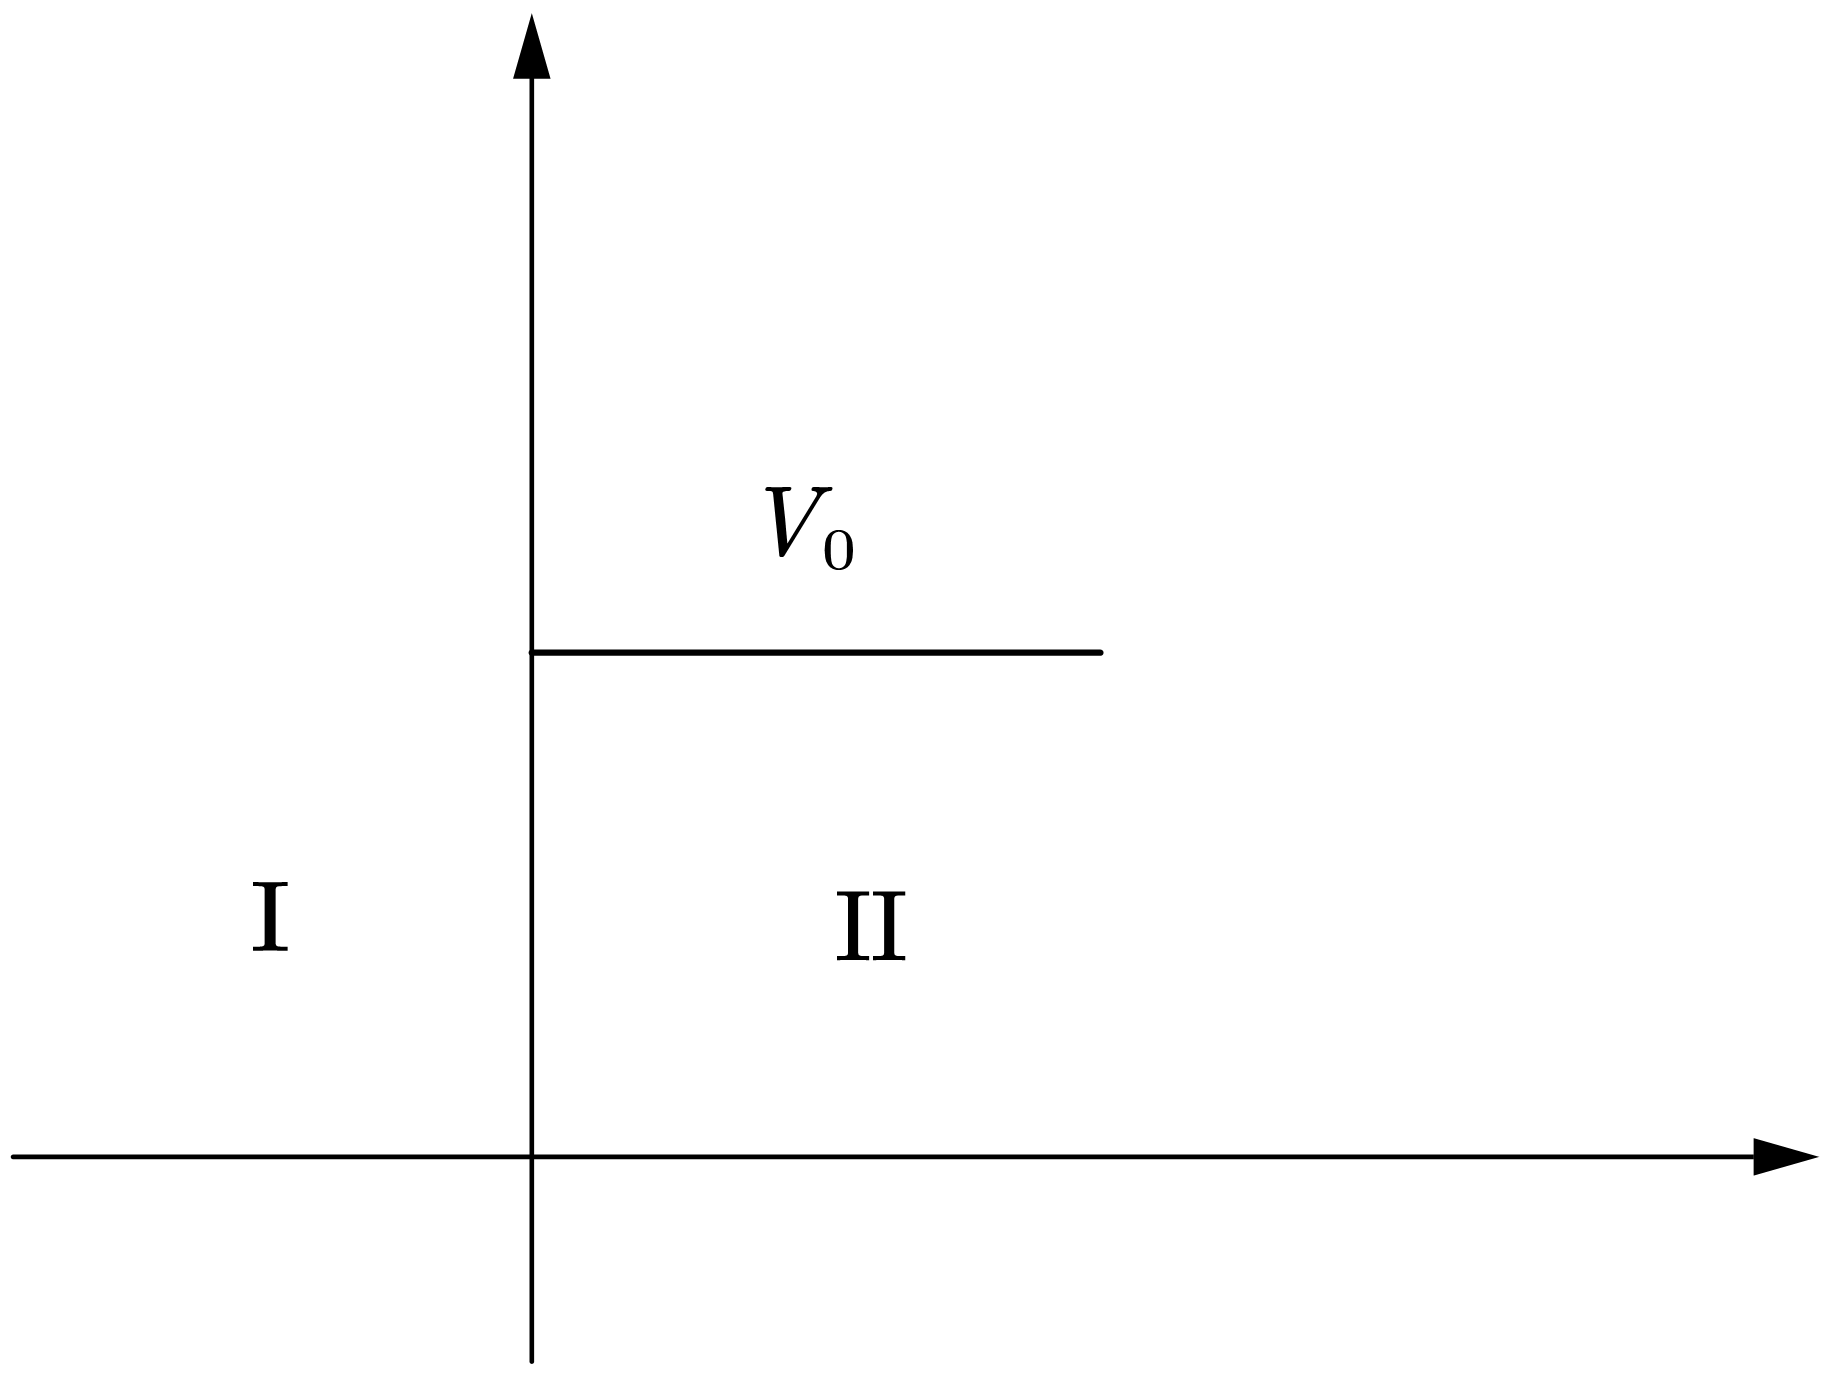
\includegraphics[width=10cm]{figure/jump-potential.png}
\end{center}
假设粒子从左向右运动,在I区域,波动方程为
\begin{equation}
\pdv[order=2]{\psi_1(x)}{x}+\frac{2m}{\hbar^2}E\psi_1(x)=0
\end{equation}
通解为
\begin{equation}
\psi_1(x)=A_1e^{ik_1x}+B_1e^{-ik_1x},k_2=\sqrt{\frac{2mE}{h^2}}
\end{equation}
假设$E<V_0$,区域II的方程为
\begin{equation}
\pdv[order=2]{\psi_2(x)}{x}-\frac{2m}{\hbar^2}(V_0-E)\psi_2(x)=0
\end{equation}
通解
$$\psi_2(x)=A_2e^{k_2x}+B_2e^{-k_2x},k_2=\sqrt{\frac{2m(V_0-E)}{\hbar^2}}$$
定解条件有3个:
\begin{enumerate}
\item 波函数有界。于是$A_2=0$。
\item 波函数在$x=0$处连续。于是$\psi_1(0)=\psi_2(0)$,有
\begin{equation}
A_1+B_1=B_2
\end{equation}
\item 由于二阶导存在,则一阶导连续,有$\psi_1'(0)=\psi_2'(0)$,即
\begin{equation}
ik_1A_1-ik_1B_1=-k_2B_2
\end{equation}
结合上一个条件,解得
\begin{empheq}{align}
B_1&=\frac{k_1^2-2k_1k_2i-k_2^2}{k_1^2+k_2^2}A_1\label{jump-model-sol-B1}\\
B_2&=\frac{2k_1^2-2k_1k_2i}{k_1^2+k_2^2}A_1
\end{empheq}
\item 归一化条件。
\begin{empheq}{equation}
\int_{-\infty}^{0}\left|A_1e^{ik_1x}+B_1e^{-ik_2x}\right|^2\dif x+\int_{0}^{\infty}\left|B_2e^{-k_2x}\right|^2\dif x
=1
\end{empheq}
这里可以使用\eqref{complex-sum-abs},可得
\begin{empheq}{equation}
\int_{-\infty}^{0}(A_1+B_1)^2-4A_1B_1\sin^2k_1 x\dif x-B_2^2
\end{empheq}
\end{enumerate}